\documentclass[a4paper,11pt]{article}
\usepackage[T1]{fontenc}
\usepackage{hyperref}
\usepackage{titlesec}
\usepackage{tipa}
\usepackage[labelfont=bf]{caption}
\usepackage{graphicx}				         % use graphicx package for images
\graphicspath{ {images/} }			         % path to images directory for the images
\renewcommand{\figurename}{Fig.}             % reconfigure caption Figure X. --> Fig. X, with X being a number.
%\titleformat{\subsection}
%[display]
%{\large\bfseries}
%{Exercise \thesubsection}{1pt}{}

% Star to kill indentation of following par.
%\titlespacing*{\subsection}
%{0pt}{5pt}{-15pt}

%\titleformat{\subsection}
%{\large\bfseries}
%{Pattern \thesubsection}{1pt}{}

\titleformat{\section}
[runin]
{\LARGE\bfseries}
{Exercise \thesection: \rightmark}{1pt}{}

\titleformat{\subsection}
{\normalfont\Large\bfseries}
{\thesubsection\hskip 5pt\textpipe\hskip 5pt}{0pt}{}


% Star to kill indentation of following par.
\titlespacing*{\subsection}
{0pt}{5pt}{0pt}

\title{TI2206 Software Engineering \\ Bubble Shooter report: Assignment 2 \\ EEMCS/EWI}
\author{Gerlof Fokkema 4257286 \\
	Owen Huang 4317459 \\
	Adam Iqbal 4293568 \\
	Nando Kartoredjo 4271378 \\
	Skip Lentz 4334051 \\
}

\begin{document}
\maketitle
\thispagestyle{empty}

\newpage
\setcounter{page}{1}

%###################################### EXERCISE 1 ###################################### 
\section{Simple Logging \\}
In this section the process of how logging is implemented in the project is explained fully in depth. \\\\
\noindent
\textbf{Responbility Driven Design in logging} \\
\noindent
In order to include logging in the project, it is important to carefully think again about the different responsibilities every class carries. It is also important to know what to log and what not to. Some things are simply not necessary to log; knowing what buttons on the main menu were pressed for example is not something of upmost importance. Other things regarding the game are much more interesting to know or estabilishing a connection with another player in multi-player. Since most game logic is put together in one class called \textit{BSMode}, having all the elements that we wish to observe one could apply the observer pattern to \textit{BSDrawable}. This causes everything that is drawable, including most things that change to be observable. By creating a class \textit{Loggable} which extends the \textit{Java Observable} class, we can therefore let any class that needs to be Observable extend our \textit{Loggable} class. The various observers are then of course added in the \textit{BSMode} class, as earlier mentioned it contains all the crucial game elements (such as cannon and board). Now we introduce another class, called the \textit{Logger} which will act as the Observer. This class will also implement the \textit{Java Observer interface}. It will contain the \textit{update} method, being called when the Observer is notified by its Observables. It is also possible to a step further, to include different kinds of logging: printing to console and to file. For this a new pattern may be introduced, a suitable pattern is for example the \textit{Strategy} pattern. This takes care of being able to include independant kinds of logging. A visual depiction of the implementation of the logger can be found below in \textbf{Fig. 1}.
\begin{minipage}{\linewidth}
\makebox[\linewidth]{
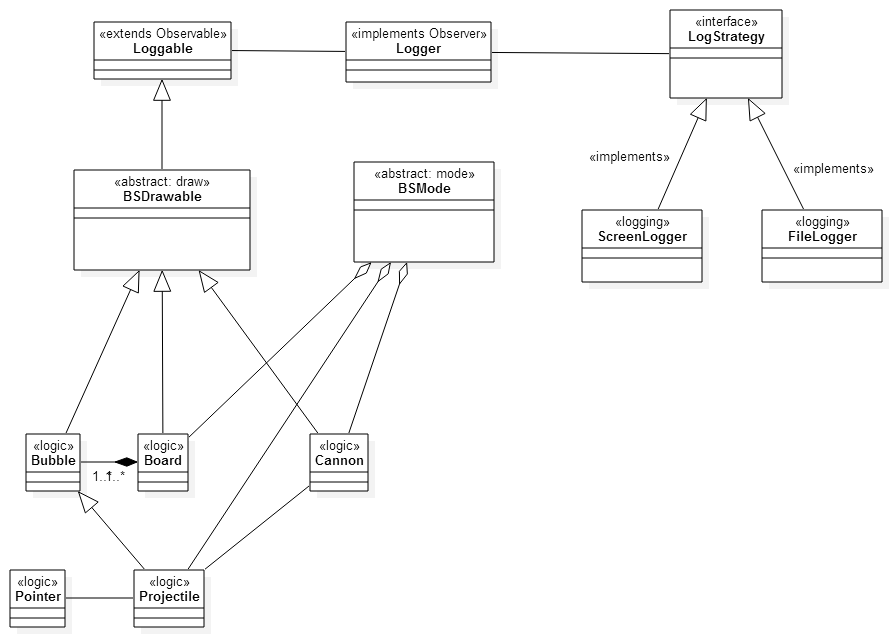
\includegraphics[width = \textwidth]{class_diagram_logging}
}
\captionof{figure}{Global layout of the implementation of the logger}
\end{minipage}
%###################################### EXERCISE 2 ###################################### 
\section{Design Patterns \\}
In this section three design patterns are elaborated with fully in depth explanations. Furthermore these patterns come with a visual depiction of how they were implemented in the project. \\

%~~~~~~~~~~~~~~~~~~~~~ Design Pattern 1 ~~~~~~~~~~~~~~~~~~~~~~
\subsection{Pattern 1: Observer for Statistics}
\begin{enumerate}
\item For the first design pattern, an \textit{Observer} pattern was chosen for the statistics of the game. For example, a single-player game contains a \textit{score} and a \textit{timer}. These elements are constantly updated throughout the game, given that something has changed about them. A \textit{timer} should count down in a continuous fashion, meanwhile the \textit{score} should only be updated when the user has gained points. These are triggerable events.
The timer is triggered by a change in time and the score by removing bubbles. So it makes sense to use something like an \textit{Observer} pattern, since it will only notify the \textit{Observer} when the \textit{Observable} triggered something and notifies the \textit{Observer} about it.

\item The class diagram for the \textit{Stats Observer} can be found in \textbf{Fig. 2}.
\begin{minipage}{\linewidth}
\makebox[\linewidth]{
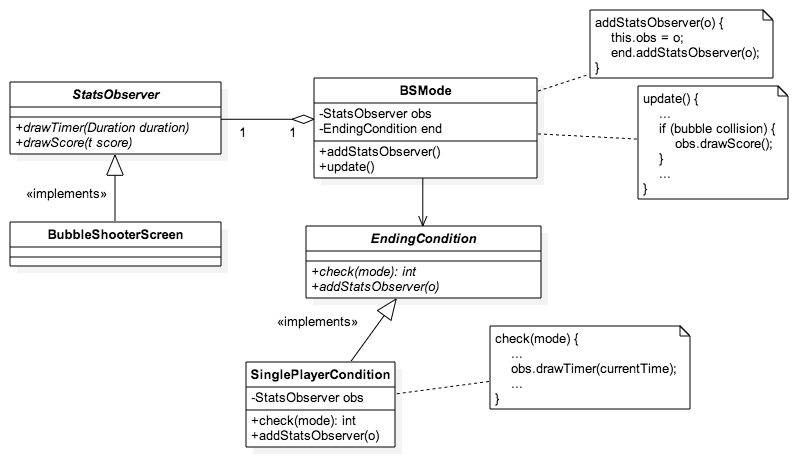
\includegraphics[width = \textwidth]{statsobserver_class}
}
\captionof{figure}{Stats Observer class diagram}
\end{minipage}
\item The sequence diagram for the \textit{Stats Observer} can be found in \textbf{Fig. 3}.
\begin{minipage}{\linewidth}
\makebox[\linewidth]{
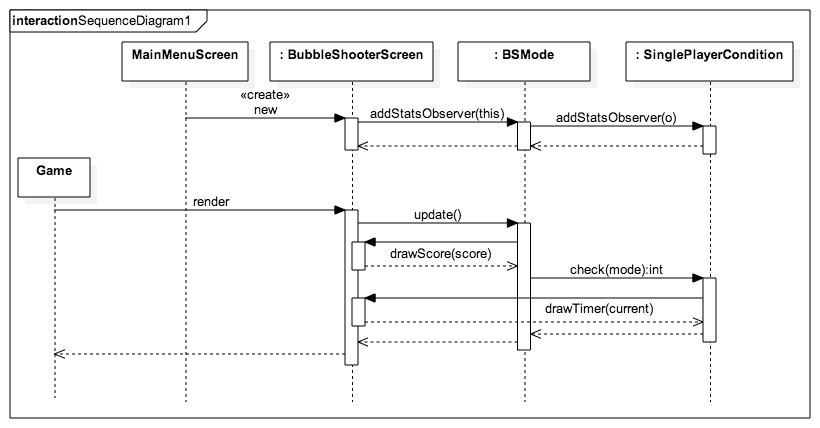
\includegraphics[width = \textwidth]{statsobserver_sequence}
}
\captionof{figure}{Stats Observer sequence diagram}
\end{minipage}
\end{enumerate}

%~~~~~~~~~~~~~~~~~~~~~ Design Pattern 2 ~~~~~~~~~~~~~~~~~~~~~~
\subsection{Pattern 2: Strategy for Ending Condition}
\begin{enumerate}
\item The second pattern we used is the \textit{Strategy} pattern, which we applied on the \textit{EndingCondition} interface, which is to be used by the \textit{BSMode} class. \\
The pattern is applied here because one should favor object composition over inheritance. We could for example have used inheritance, and make a subclass of \textit{BSMode} for each game mode. However, a lot of the game logic is the same, and really the only difference is how the  game should end.\\
Using the \textit{EndingCondition} class, we get a greater amount of flexibility: we pass the desired \textit{EndingCondition} to the constructor of a \textit{BSMode} class, and automatically the logic for the end of the game is done for us, by means of polymorphism.\\
\item
\item
\end{enumerate}

%~~~~~~~~~~~~~~~~~~~~~ Design Pattern 3 ~~~~~~~~~~~~~~~~~~~~~~
\subsection{Pattern 3: Singleton for Assets}
\begin{enumerate}
\item The Singleton pattern makes sure that there is only one instance of \textit{Assets} and it can be accessed globally. This is useful because we only need one instance of \textit{Assets} and we only need to load the assets once with the same instance. The loading happens when the application is initiated, in the very beginning before the user even sees anything. So, by applying the singleton pattern, it provides easy access for the class responsible for the initial launching of the application.
\item
\item
\end{enumerate}


%###################################### EXERCISE 3 ###################################### 
\section{Optional - One more design pattern \\}
In this section an additional design pattern is implemented and elaborated.
%~~~~~~~~~~~~~~~~~~~~~ Extra Pattern 3 ~~~~~~~~~~~~~~~~~~~~~~
\subsection{Pattern 3:  Observer for Networking}
\begin{enumerate}
\item For the third pattern, we chose to use the \textit{Observer} pattern again to improve our networking code. \\
When playing against another player, the remote client only has to know about changes in the current state of the host.
Therefore it makes sense to use the \textit{Observer} pattern for sending our state to the remote client. \\
We were able to improve networking performance by changing all \textit{BSDrawable} objects into \textit{Observable} objects and by letting the \textit{MultiPlayerMode} class listen to changes made to them.
Now the \textit{MultiPlayerMode} only sends \textit{BSDrawable} objects over the network when they have changed.
\item The class diagram for the \textit{Networking Observer} can be found in \textbf{Fig. TBD}. \\
\begin{minipage}{\linewidth}
\makebox[\linewidth]{
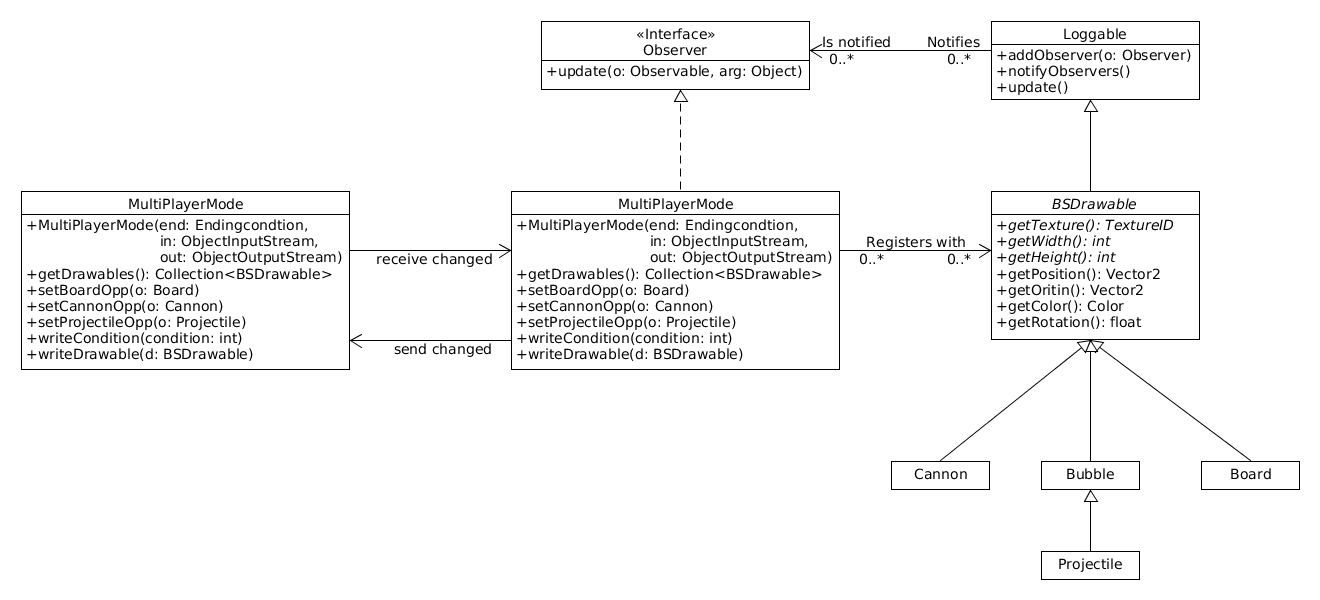
\includegraphics[width = \textwidth]{networking}
}
\captionof{figure}{Networking Observer class diagram}
\end{minipage}
\item
\end{enumerate}

\end{document}